%
% 2-homogen.tex
%
% (c) 2023 Prof Dr Andreas Müller
%
\section{Homogene Räume
\label{buch:nichtkomm:section:homogeneraeume}}
\kopfrechts{Homogene Räume}
Im vorangegangenen Abschnitt haben wir eine gemeinsame mathematische
Formalisierung für verschiedene Varianten des Registrierungsproblems
gefunden.
In diesem Abschnitt wenden wir uns den Gemeinsamkeiten des 
abstrakten Problems zu und ermitteln die Struktur, die uns später
helfen wird, das Registrierungsproblem auf einheitliche Weise
in einfachere Teilprobleme aufzuteilen.

%
% Stabilisator
%
\subsection{Stabilisator
\label{buch:nichtkomm:homogen:subsection:stabilisator}}
In die grosse Menge der Transformationen des Definitionsbereiches
$X$ lässt sich etwas Ordnung bringen, indem man Fixpunkte dieser
Transformationen sucht.
\index{Fixpunkt}

\begin{definition}[Fixpunkt, Stabilisator]
Wenn die Gruppe $G$ auf dem Raum $X$ operiert und $x\in X$ ist, dann
heisst $x$ ein {\em Fixpunkt} einer Transformation $s\in G$, wenn 
\index{Fixpunkt}%
$s\cdot x = x$ ist.
Die Menge
\[
S_x = \{ s\in G \mid s\cdot x = x \}
\]
aller Transformationen, die $x$ als Fixpunkt haben,
heisst der {\em Stabilisator} von $x$.
\index{Stabilisator}%
\end{definition}

Der Stabilisator eines Punktes $x\in X$ ist immer eine Untergruppe.
Dazu muss man nur überprüfen, ob die Zusammensetzung und die Inverse
von Elementen aus $S_x$ wieder in $S_x$ liegt.
Dies ist aber klar, denn wenn zwei Elemente $g,h\in S_x$ den Punkt $x$
festhalten, dann ist auch $(gh)\cdot x= g\cdot(h\cdot x) = g\cdot x = x$
und analog für die Inverse.

\begin{beispiel}
\label{buch:nichtkomm:homogen:bsp:SO3}
Die Gruppe $\operatorname{SO}(2)\ltimes\mathbb{R}^2$ operiert auf der
Mengen $X=\mathbb{R}^2$.
Nicht jede Transformation hat einen Fixpunkt, zum Beispiel haben reine
Verschiebungen um einen Vektor $v\in\mathbb{R}^2$, $v\ne 0$, keinen
Fixpunkt.
Für eine Transformation $(s,a)\in\operatorname{SO}(2)\ltimes \mathbb{R}^2$
mit $s\ne e$, also eine Transformation mit einer nichttrivialen
Drehkomponente, lässt sich immer ein Fixpunkt durch Lösung der 
Gleichung
\[
sx+a=x
\quad\Rightarrow\quad
x = -(s-e)^{-1}a
\]
ermitteln.
Diese Lösung ist genau dann möglich, wenn $s-e$ invertierbar ist.
Ob eine Matrix invertierbar ist,
kann mit der Determinante entschieden werden.
Die Determinante der Matrix $D_\alpha-I$ ist
\begin{align*}
\det(D_\alpha-I)
&=
(\cos\alpha-1)^2+\sin^2\alpha
\\
&=
\cos^2\alpha-2\cos\alpha +1+\sin^2\alpha
\\
&=
2-2\cos\alpha 
\\
&=
2(1-\cos\alpha).
\end{align*}
Diese verschwindget genau dann, wenn $\alpha$ ein Vielfaches von $2\pi$ ist.
Damit ist gezeigt, dass alle Transformationen mit einer nichttrivialen
Drehkomponente einen Fixpunkt haben.

Der Stabilisator eines Punktes $x\in\mathbb{R}$ besteht aus denjenigen
$(g,a)\in\operatorname{SO}(2)\ltimes \mathbb{R}^2$, für die
\[
(g,a)\cdot x = g\cdot x+a = x
\]
gilt.
Daraus leitet man die Bedingung 
\[
(g-e)\cdot x = -a
\]
ab.
Für jede Drehung $g\in\operatorname{SO}(2)$ gibt es also einen Vektor
$a=-(g-e)$ derart, dass $(g,a)\in\operatorname{SO}(2)\ltimes\mathbb{R}^2$
den Punkt $x$ als Fixpunkt hat.
Die Abbildung $g\mapsto(g,-gx+x)$ ist daher ein Isomorphismus von
$\operatorname{SO}(2)$ auf den Stabilisator
$S_x\subset \operatorname{SO}(2)\ltimes \mathbb{R}^2$.
\end{beispiel}

\begin{beispiel}
Die Gruppe $G=\operatorname{SO}(3)$ operiert auf der Kugeloberfläche $S^2$.
Der Stabilisator eines Punktes $x\in S^2$ auf der Kugeloberfläche besteht
aus allen Drehungen, die die Achse mit Richtung $x$ oder $-x$ fest
lassen.
Die Untergruppe der Drehungen um die Achse ist isomorph zur Gruppe der
zweidimensionalen Drehmatrizen.
Ein Isomorphismus kann wie folgt konstruieren.
Zunächst wählt man zwei Einheitsvektoren $b_1,b_2\in \mathbb{R}^3$ derart,
dass $b_1,b_2$ und $x$ eine orthonormierte Basis bilden.
In dieser Basis können Drehungen $s$ um die Achse $x$ durch Matrizen der Form
\begin{equation}
s
=
\left(
\begin{array}{cc|c}
\cos\alpha & -\sin\alpha & 0 \\
\sin\alpha &  \cos\alpha & 0 \\
\hline
     0     &       0     & 1
\end{array}
\right)
=
\left(
\begin{array}{cc|c}
\multicolumn{2}{c|}{
\multirow{2}{*}{$D_\alpha$}
}&0\\
&&0\\
\hline
0&0&1
\end{array}
\right)
\quad\text{mit}\quad
D_\alpha\in\operatorname{SO}(2)
\label{buch:nichtkomm:homogen:bsp:SO3:op}
\end{equation}
dargestellt werden.
Die Abbildung $D_\alpha\mapsto s$ ist ein Isomorphismus von
$\operatorname{SO}(2)$ auf den Stabilsator $S_x\subset\operatorname{SO}(3)$.
\end{beispiel}

%
% Homogener Raum
%
\subsection{Homogener Raum
\label{buch:nichtkomm:homogen:subsection:homogen}}
Die Definitionsgebiete $X$, die wir im Registrierungsproblem untersuchen,
haben noch eine zusätzliche Eigenschaft.
Für jedes Paar von Punkten $x$ und $y$ in $X$ lässt sich immer mindestens
eine Transformation $g\in G$ finden derart, dass $g\cdot x = y$ ist.
Man sagt, die Gruppe $G$ operiert {\em transitiv} auf $X$.

Typischerweise gibt es nicht nur ein Gruppenelement $g$, welches $x$ in
$y$ transportiert.
Ist $s\in S_x$, dann ist auch $gsx=gx=y$ und für $t\in S_y$ ist
auch $tgx=ty=y$.

\begin{satz}
Falls $gx=hx=x$, dann gibt es eine Element $s\in S_x$ derart, dass
$gs=h$.
\end{satz}

\begin{proof}[Beweis]
Aus $gx=hx$ folgt $x=g^{-1}hx$, also $s=g^{-1}h\in S_x$.
Ausserdem ist $gs=gg^{-1}h=h$, wie verlangt.
\end{proof}

\begin{satz}[Isomorphie der Stabilisatoren]
Wenn die Gruppe $G$ transitiv auf dem Raum $X$ operiert und $x,y\in X$
zwei Punkte in $X$ sind, dann sind die Stabilisatoren $S_x$ und $S_y$
isomorph.
Ist $gx=y$ dann ist die Abbildung
\[
c_g\colon
S_y\to S_x: h\mapsto ghg^{-1}
\]
ein Isomorphismus der Stabilisatoren.
\end{satz}

\begin{proof}[Beweis]
Zunächst können wir leicht nachrechnen, dass $c_g$ ein Homomorphismus ist,
denn
\[
c_g(hk)
=
ghkg^{-1}
=
gh(g^{-1}g)kg^{-1}
=
(ghg^{-1})gkg^{-1})
=
c_g(h)c_g(k).
\]
Wir müssen überprüfen, dass $c_g(s)\in S_y$ ist, wenn $s\in S_x$ ist.
Dazu rechnen wir nach, dass
\begin{equation}
c_g(s)y = gsg^{-1} y = gsx=gx=y
\quad\Rightarrow\quad
c_g(s)\in S_x.
\label{buch:nichtkomm:homogen:eqn:cgimage}
\end{equation}
Der Homomorphismus $c_g$ ist aber auch umkehrbar, denn es gilt
\[
c_gc_{g^{-1}}(h)
=
g(g^{-1}hg)g^{-1}h
=
h
\quad\Rightarrow\quad
c_gc_{g^{-1}}=\operatorname{id}.
\]
Aus \eqref{buch:nichtkomm:homogen:eqn:cgimage} folgt jetzt, dass
$c_{g^{-1}}\colon S_y\to S_x$.
Somit ist $c_g$ ein Isomorphismus.
\end{proof}

Der Satz besagt also, dass in jedem Punkt des Raumes $X$ der gleiche
Stabilisator gefunden wird.
Mit den  Mitteln der Gruppentheorie von $G$ lassen sich zwei Punkte 
in $X$ nicht unterscheiden.
Diese spezielle Situation hat einen Namen.

\begin{definition}[homogener Raum]
Ein Raum $X$, auf dem eine Gruppe $G$ transitiv wirkt, heisst
{\em homogen}, wenn der Stabilisator in jedem Punkt von $x$ gleich ist.
\index{homogen}%
\index{homogener Raum}%
\end{definition}

Da die Gruppe $G$ transitiv auf $X$ wirkt, kann man die Punkte $y$ von 
$X$ auch durch die Transformationen bechreiben, die einen gewählten
Punkte $x$ in $y$ überführen.
Die Tatsache, dass der Stabilisator in jedem Punkt isomorph ist, 
bedeutet, dass der Raum in jedem Punkt ``gleich aussieht'', er hat
hat dort die gleiche Symmetriegruppe.
Ein homogener Raum ist also ein Raum mit einer Gruppenoperation derart,
dass alle Punkte isomorphe Symmetrieuntergruppen haben.

\begin{beispiel}
Sei $x$ der Nordpol der zweidimensionalen Kugeloberfläche $S^2$.
Ist $y\in S^2$ ein weiterer Punkt, gibt es eine Drehung um die Achse,
die durch das Vektorprodukt
$x\times y$ gegeben ist.
Sie transportiert den Nordpol in den Punkt $y$ transportiert.
Alle anderen Drehungen, die den Nordpol in den Punkt $y$ überführen,
bestehen aus einer Drehung um die Nord-Süd-Achse gefolgt von der
genannten Drehung um $x\times y$.
\end{beispiel}

%
% Der Quotientenraum
%
\subsection{Der Quotientenraum $G/K$
\label{buch:nichtkomm:homogen:subsection:quotientgk}}
Sie $G$ eine topologische Gruppe und $K$ eine Untergruppe, die auf $G$
von rechts wirkt.
Zu jedem Element $g\in G$ ist $gK$ die Menge aller Gruppenelemente, 
die mit Hilfe der Rechtsoperation mit einem Element von $K$ erreicht
werden können.
$gK$ heisst auch der {\em Rechtsorbit} oder einfach {\em Orbit} von $g$
bezüglich der Operation von $K$ auf $G$ von rechts.

\begin{definition}[Orbitraum]
Die Menge 
\[
G/K
=
\{ gK \mid g\in G\}
\]
heisst der {\em Orbitraum} der Wirkung von $K$ auf $G$.
\end{definition}

%
% Grenzwertbegriff auf G/K
%
\subsubsection{Grenzwertbegriff auf $G/K$}
Es ist nicht selbstverständlich, dass der Orbitraum
mit einem brauchbaren Grenzwertbegriff ausgestattet
werden kann.

\begin{beispiel}
Die Gruppe $\mathbb{Z}\subset\mathbb{R}$ ist abelsch, der Orbit einer
Zahl $x\in\mathbb{R}$ besteht aus allen Zahlen, die den gleichen
Nachkommateil haben wie $x$.
Sie können dargestellt werden durch die Zahlen im halboffenene
Intervall $[0,1)$.
Die Folge $x_n = 1-1/n\in [0,1)$ konvergiert gegen $1$, was im gleichen
Orbit wie $0$ liegt.
Als topologischer Raum muss man den Orbitraum also mit den
Punkten einer Kreislinie, die man zum Beispiel durch die
Parametrisierung $\mathbb{R}\to S^1:x\mapsto e^{2\pi ix}$ 
beschreiben kann, die $\mathbb{R}$ surjektiv auf $S^1$ abbildet.
\end{beispiel}

Der Orbitraum des vorangegangenen Beispiels der reellen Zahlen
modulo $\mathbb{Z}$ ist sogar eine Gruppe.

\begin{beispiel}
Sei $G=\mathbb{R}/\mathbb{Z}$,
$\alpha\in [0,1)$ eine beliebige Zahl und $K=\alpha\mathbb{Z}$
die Menge aller Vielfachen von $\alpha$ in $G$.
$K$ ist eine Untergruppe von $G$.
Die Menge $K$ ist abzählbar unendlich aber $G$ ist überabzählbar,
der Orbitraum muss also überabzählbar unendlich sein.

Ist $\alpha\in\mathbb{Q}$, dann sei $\alpha=p/q$ die Darstellung
von $\alpha$ als gekürzter Bruch.
Da $q\alpha=p$ ganzzahlig ist, gilt in $G$, dass $q\alpha=0$ ist.
Da der Bruch gekürzt ist, ist $q$ die kleinste Zahl mit dieser
Eigenschaft.
Die Untergruppe $K$ ist in diesem Fall die $q$-elementige endliche
Untergruppe
\[
K = \biggl\{ \frac1qk \;\bigg|\; k=0,\dots,q-1 \biggr\}
\]
von $G$.
Die Orbits von $G/K$ bestehen aus den Elementen, die gleich grossen
Unterschied zum nächstkleineren Element von $K$ aufweisen.
Die Abbildung $q\colon G \to G: x\mapsto qx$ bildet die ganze
Untergruppe $K$ auf $0$ ab und das Intervall $[0,\frac1q)$ auf
$[0,1)$, was zeigt, dass $G/K$ wie $G$ selbst eine Kreislinie ist.

Ist $\alpha\not\in \mathbb{Q}$, dann sind die ganzzahligen Vielfachen
von $\mathbb{Q}$ alle verschieden und bilden eine Untergruppe von $G$,
die jedem Element von $G$ beliebig nahe kommt.
Der Orbitraum ist zwar immer noch eine überabzählbar unendliche
Menge, aber es ist nicht möglich, einen sinnvollen Grenzwertbegriff
zu konstruieren.
Die Folge der Zahlen $x_k=k\alpha$ kommt zwei beliebigen Elementen
von $G$ immer wieder beliebig nahe, sie müssten daher auch in $G/K$
als beliebig nahe beeinander betrachtet werden.
\end{beispiel}

Der Unterschied zwischen den Fällen $\alpha\in\mathbb{Q}$ und
$\alpha\not\in\mathbb{Q}$ äussert sich in der Tatsache, dass
die von $\alpha$ erzeugte Teilmenge $\alpha\mathbb{Z}\subset G$ 
im ersten Fall eine abgeschlossene Teilmenge von $G$ ist,
im zweiten Fall aber nicht.
Dies wird auch durch das folgende Beispiel illustriert.

\begin{beispiel}
Sei $G=\mathbb{R}^2/\mathbb{Z}^2 = (\mathbb{R}/\mathbb{Z})^2$,
also Paare von Elementen der additiven abelsche Gruppe der reellen
Zahlen modulo $\mathbb{Z}$ wie im vorangegangenen Beispiel.
Sei ausserdem $K=\{(k,\alpha k)\mid k\in\mathbb{R}\}\subset G$
die Untergruppe, die durch die Konstante $\alpha$ definiert wird.
Je nachdem ob $\alpha$ rational oder irrational ist, ist die Menge der
Orbits völlig verschieden.

Ist $\alpha\in\mathbb{Q}$, dann gibt es eine Darstellung $\alpha=p/q$
als gekürzter Bruch.
Dies bedeutet, dass $K$ als Teilmenge von $[0,1)$ aus $q$ parallelen
Strecken besteht.
Die Orbits von $K$ bestehen aus den Punkten von $[0,1)$, die gleich weit
vom nächsten ``darunterliegenden'' Geradenstück entfernt sind.
Der Orbitraum ist also wieder $\mathbb{R}/\mathbb{Z}$.

Ist $\alpha\not\in\mathbb{Q}$, dann kommt $K$ jedem Punkt von $G$ beliebig
nahe, $K$ ist also nicht abgeschlossen in $G$ und wie im vorangegangenen
Beispiel ist lässt sich kein nützlicher Grenwertbegriff definieren.
\end{beispiel}

Wir schränken daher im folgenden die Verwendung des Begriffs des
Orbitraums $G/K$ auf Fälle ein, in denen die Untergruppe $K$ eine
abgeschlossene Untergruppe von $G$ ist.
Diese Bedingung ist insbesondere dann immer erfüllt, wenn $K$ eine
kompakte Untergruppe ist.

%
% Linksorbits
%
\subsubsection{Linksorbits}
Alle Begriffe, die im vorangegangenen Abschnitt für die Rechtsoperation
der Untergruppe $K$ auf $G$ entwickelt wurden, lassen sich genauso
auch für die Linksoperation von $K$ auf $G$ entwicklen.
Der zugehörige {\em Links-Orbitraum} ist die Menge
\[
K\backslash G
=
\{ Kg \mid g\in G \},
\]
wie im Falle von $G/K$ kann sie nur dann mit einem nützlichen
Grenzwertbegriff versehen werden, wenn $K$ abgeschlossen ist.

\begin{beispiel}
\label{buch:nichtkomm:homogen:bsp:so2r2}
\begin{figure}
\centering
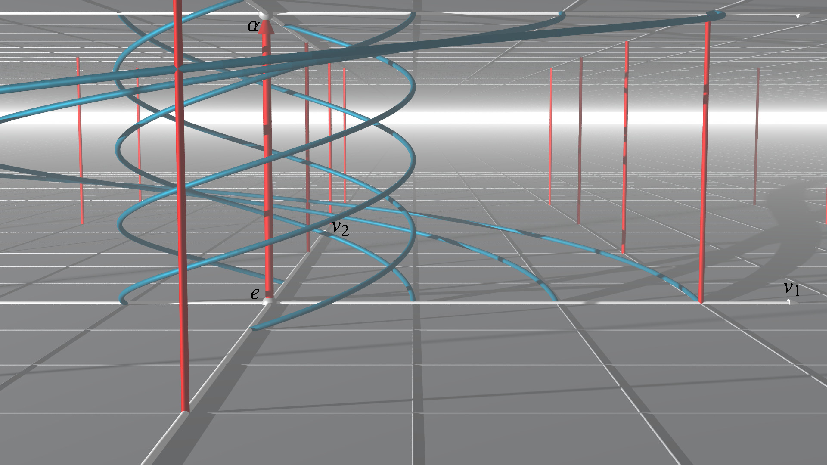
\includegraphics{chapters/070-nichtkomm/images/so2r2.pdf}
\caption{Visualisierung der Gruppe $\operatorname{SO}(2)\ltimes \mathbb{R}^2$
als dreidimensionale Mannigfaltigkeit.
Die Ebene aufgespannt von den Vektoren $v_1$ und $v_2$ ist der Faktor
$\mathbb{R}^2$.
Die Drehungen in $\operatorname{SO}(2)$ werden parametrisiert durch
die auf der vertikalen Achse abgetragenen Drehwinkel $\alpha$, die 
aus dem Intervall $[0,2\pi)$.
Die roten und blauen Kurven zeigen die Rechts- bzw.~Linksorbits
(siehe Beispiel~\ref{buch:nichtkomm:homogen:bsp:so2r2}).
\label{buch:nichtkomm:homogen:fig:so2r2}}
\end{figure}
Die Gruppe $G=\operatorname{SO}(2)\ltimes \mathbb{R}^2$ ist in 
Abbildung~\ref{buch:nichtkomm:homogen:fig:so2r2} visualisiert.
Die horizontalen Ebenen mit Basisvektoren $v_1$ und $v_2$ 
entsprechen dem Faktor $\mathbb{R}^2$.
Auf der vertikalen Achse ist der Drehwinkel $\alpha$ einer Drehung
im Faktor $\operatorname{SO}(2)$ des semidirekten Produktes abgetragen.

Die Elemente $s\subset \operatorname{SO}(2)=K$ werden als Paare
$(s,0)\in \operatorname{SO}(2)\ltimes\mathbb{R}^2$ eingebettet.
Die Rechtsorbits der Operation von $\operatorname{SO}(2)$ auf
$\operatorname{SO}\ltimes \mathbb{R}^2$ sind daher die roten vertikalen
Linien in der Abbildung.
Der Orbitraum
$G/K
=
\operatorname{SO}(2)\ltimes\mathbb{R}^2/\operatorname{SO}(2)$
kann daher mit der Ebene identifiziert werden.

Die Multiplikation mit einer Drehung $s$ mit Drehwinkel $\alpha$ von
Links fügt der ersten Komponente eines Elements $(t,v)$ von
$\operatorname{SO}(2)\ltimes\mathbb{R}^2$ den Drehwinkel hinzu, 
verschiebt den zugehörigen Punkt in
Abbildung~\ref{buch:nichtkomm:homogen:fig:so2r2}
Punkt um $\alpha$ nach oben.
Auf der Vektorkomponente $v$ wirkt $s$ dagegen als Drehung.
So entstehen die blauen Spiralen in
Abbildung~\ref{buch:nichtkomm:homogen:fig:so2r2}
als
Linksorbits der Wirkung von $\operatorname{SO}(2)$ auf $G$.
\end{beispiel}

%
%  Homogene Räume als Quotientenräume
%
\subsubsection{Homogene Räume als Quotientenräume}
Wir betrachten einen homogenen Raum $X$, auf dem die Gruppe $G$
transitiv wirkt.
Sei $x\in X$ ein Punkt von $X$ und $S_x$ der Stabilisator des
Punktes $x$.
Wir betrachten die Abbildung
\[
f
\colon
G\to X
:
g \mapsto x.
\]
Sie ist surjektiv, weil die Gruppe transitiv auf $X$ wirkt und
daher jeden beliebigen Punkt von $x$ aus erreichen kann.

Die Untergruppe $S_x\in G$ operiert durch Rechtsoperation auf $G$.
Wegen $sx=x$ für $s\in S_x$ gilt für die Elemente des Orbits
$gS_x$, dass sie den Punkt $x$ alle auf den gleichen Punkt
\(
gsx = gx
\)
abbilden.
Die Abbildung $f$ bildet daher $S_x$-Orbits bijektiv auf die
Punkte von $X$ ab.

\begin{satz}
\label{buch:nichtkomm:homogen:satz:homorbitraum}
Ist $X$ ein homogener Raum, auf dem die Gruppe $G$ durch Linksoperation
transitiv wirkt, und ist $S_x$ der Stabilisator eines Punktes $x$, dann
ist die Abbildung
\[
f
\colon
G/S_x \to  X
:
gS_x \mapsto gx
\]
ein Homöomorphismus.
\end{satz}

Der Satz zeigt, dass es gar nicht nötig ist, abstrakte homogene Räume
zu betrachten, da solche immer als Orbitraum einer Gruppenoperation 
konstruiert werden können.

\begin{beispiel}
\label{buch:nichtkomm:homogen:bsp:SO3/SO2}
Im Beispiel~\ref{buch:nichtkomm:homogen:bsp:SO3} wurde gezeigt,
die Gruppe $\operatorname{SO}(3)$ transitiv auf der Kugeloberfläche
$S^2$ wirkt und dass der Stabilisator des Nordpols der Kugel
eine Untergruppe $\operatorname{SO}(2)\subset\operatorname{SO}(3)$ ist.
Aus Satz~\ref{buch:nichtkomm:homogen:satz:homorbitraum} folgt nun,
dass die Kugel $S^2\cong \operatorname{SO}(3)/\operatorname{SO}(2)$
ist.
Orbits bestehen aus den orthogonalen Matrizen, die sich nur durch
Multiplikation mit einer Matrix $s$ wie in 
\eqref{buch:nichtkomm:homogen:bsp:SO3:op}
unterschieden.
Ein Matrix in $\operatorname{SO}(3)$ besteht aus orthonormierten 
Zeilen, von denen die letzte bei Multiplikation mit $s$ fest bleibt.
Die ersten zwei Zeilen sind orthogonal auf der dritten und werden durch
$s$ ineinander übergeführt.
Die Orbits bestehen also aus den orthogonalen Matrizen mit der gleichen
letzten Zeile.
\end{beispiel}

%
% Gruppenoperation auf $G/K$
%
\subsubsection{Gruppenoperation auf $G/K$
\label{buch:nichtkomm:homogen:subsection:opaufgk}}
Der Satz~\ref{buch:nichtkomm:homogen:satz:homorbitraum} zeigt, dass
ein homogener Raum $X$ als topologischer Raum immer mit dem Orbitraum
$G/S_x$ identifiziert werden kann, wobei $S_x\subset G$ ein abgeschlossene
Untergruppe ist.
Aber auch die Gruppenoperation der Gruppe $G$ auf $G/S_x$ von links
stimmt mit der Operation auf $X$ überein.

\begin{beispiel}
In Beispiel~\ref{buch:nichtkomm:homogen:bsp:SO3/SO2} wurde darauf
hingewiesen, dass die Kugeloberfläche $S^2$ der homogene Raum
$\operatorname{SO}(3)/\operatorname{SO}(2)$ ist.
Die Orbits bestehen aus orthogonalen Matrizen mit der gleichen letzten
Zeile.
Die Multiplikation mit einer Matrix $s$ wie in 
\eqref{buch:nichtkomm:homogen:bsp:SO3:op}
ist eine Drehung der Kugel um die vertikale Achse.
\end{beispiel}

%
% Registrierungsproblem
%
\subsubsection{Registrierungsproblem für ein Paar von Gruppen}
Das Registrierungsproblem für Bilder in einer Ebene besteht
darin, ein Element von $G=\operatorname{SO}(2)\ltimes \mathbb{R}^2$
zu finden, welches zwei Funktionen in der Ebene $X=\mathbb{R}^2$
zur Deckung bringt.
Die Gruppe wirkt aber transitiv auf $X$ mit Stabilisator
$\operatorname{SO}(2)$, also ist $X$ ein homogener Raum.
Wegen $X=\operatorname{SO}(2)\ltimes\mathbb{R}^2/\operatorname{SO}(2)$
wird das Registrierungsproblem vollständig durch die Angabe
der Gruppe $G=\operatorname{SO}(2)\ltimes \mathbb{R}^2$ und
die abgeschlossene Untergruppe $\operatorname{SO}(2)$ festlegt.

Beim Registrierungsproblem für Funktionen auf der Kugeloberfläche
$S^2$ wurde ähnlich festgestellt, dass die Gruppe $\operatorname{SO}(3)$
transitiv darauf wirkt mit Stabilisator $\operatorname{SO}(2)$ und
dass $S^2\cong \operatorname{SO}(3)/\operatorname{SO}(2)$.
Auch hier spezifiziert das Paar der Gruppen $G=\operatorname{SO}(3)$
und $K=\operatorname{SO}(2)$ das Registrierungsproblem vollständig.



